\section{Dispositivos de estado sólido}
\subsection{Diodos semiconductores}

Los diodos semiconductores son dispositivos electrónicos que permiten que \textbf{la corriente eléctrica fluya en una sola dirección}, mientras que en la dirección opuesta impide el paso. Están fabricados a partir de materiales semiconductores, como el \textsl{silicio} o el \textsl{germanio}, que tienen una conductividad eléctrica intermedia entre los conductores y los aislantes.\\


El diodo semiconductor consta de dos regiones de material semiconductor dopado con impurezas de diferentes tipos, creando así una unión \textbf{PN}. La región de tipo \textbf{P} se llama ánodo, mientras que la región de tipo \textbf{N} se llama cátodo.

Cuando se aplica una tensión en la dirección correcta (es decir, en la dirección ánodo-cátodo), los electrones se mueven a través de la unión PN y fluyen a través del diodo, lo que permite que la corriente eléctrica pase a través del dispositivo. Sin embargo, cuando se aplica una diferencia de potencial en la dirección opuesta, la unión PN actúa como una barrera y la corriente eléctrica se bloquea.

Los diodos semiconductores se utilizan en una amplia variedad de aplicaciones, como la rectificación de corriente eléctrica de CA a CC, la protección contra sobretensiones, la regulación de voltaje y la generación de luz en diodos emisores de luz (LED). Además, se utilizan en dispositivos más complejos, como los transistores y los circuitos integrados.

\subsubsection{Curva característica}

La curva característica de un diodo es una representación gráfica de la relación entre la corriente y la tensión que fluyen a través del diodo en diferentes condiciones de operación.\\


El diodo de tipo PN tiene una curva que se muestra en la figura \ref{fig:cc-diodo-pn} y pueden observarse dos zonas:
\begin{itemize}
	\item \textsl{Zona de polarización directa:} el ánodo tiene aplicada una mayor tensión respecto al cátodo. Si se supera una tensión $V_f$ (característica de cada dispositivo), el diodo conduce corriente.
	\item \textsl{Zona de polarización inversa:} el cátodo tiene aplicada una mayor tensión respecto al ánodo. El diodo no conducirá corriente siempre y cuando no supere la \textsl{tensión de ruptura} o \textsl{tensión pico inversa}.
\end{itemize} 

\subsection{Diodos Zener}

Un diodo Zener es un tipo especial de diodo que \textbf{se utiliza para regular la tensión en un circuito electrónico}. A diferencia de los diodos regulares, que sólo permiten el flujo de corriente en una dirección, los diodos Zener están diseñados para \textbf{permitir el flujo de corriente en ambas direcciones} cuando la tensión aplicada alcanza un valor específico llamado \textsl{tensión de ruptura} o \textsl{tensión Zener}.\\

\begin{figure}[H]
	\centering
	\begin{subfigure}[b]{.3\linewidth}
		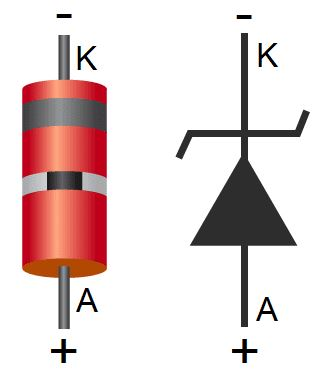
\includegraphics[width = .8\linewidth]{zener-directa}
		\caption{En directa}
		\label{fig:zener-directa}
	\end{subfigure}
	\begin{subfigure}[b]{.3\linewidth}
		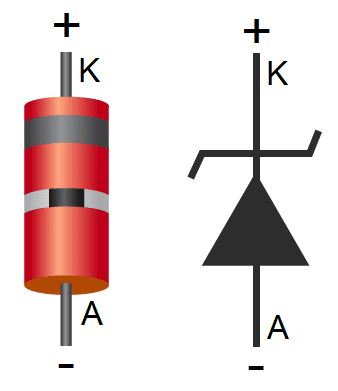
\includegraphics[width = .8\linewidth]{zener-inversa}
		\caption{En inversa}
		\label{fig:zener-inversa}
	\end{subfigure}
	\caption{Polarización del diodo zener}
\end{figure}


Cuando un diodo Zener está polarizado en inversa, como ilustra la figura \ref{fig:zener-inversa}, y se alcanza la tensión Zener, comienza a conducir corriente en la dirección opuesta, lo que permite que la tensión se mantenga constante en el circuito.

 Debido a esta propiedad, los diodos Zener se utilizan comúnmente en aplicaciones de regulación de voltaje, como fuentes de alimentación, reguladores de voltaje y circuitos de protección contra sobretensiones.